\documentclass[letterpaper, 11pt]{article}
\usepackage[margin=1in]{geometry}

% input
\usepackage[utf8]{inputenc}
\usepackage{fontspec}
\usepackage{lmodern}
\renewcommand{\familydefault}{\sfdefault}

% math
\usepackage{mathtools}

% references
\usepackage{hyperref}
\hypersetup{
    colorlinks=true,
    linkcolor=blue
}

% figures
\usepackage{tikz}
\usetikzlibrary{arrows.meta}
\usepackage{listings}
\usepackage{siunitx}
\usepackage{threeparttable}
\usepackage{lilyglyphs}
\usepackage{graphicx}
\usepackage{caption}
\usepackage[nofragment]{lyluatex}

% title
\title{Excerpts from Formalized Music}
\author{Iannis Xenakis}
\date{}

\begin{document}

\maketitle

\section*{Chapter V: Free Stochastic Music by Computer}

After this interlude, we return to the treatment of composition by machines.

The theory put forward by \textit{Achorripsis} had to wait four years before being realized
mechanically. This realization occurred thanks to M. François Génuys of IBM-France and to M. Jacques
Barraud of the Régie Autonome des Transports Parisiens.

\begin{center}
    \Large The Paradox: Music and Computers
\end{center}

\subsection*{A Stochastic Work Executed by the IBM-7090}

The general public has a number of different reactions when faced by the alliance of the machine
with artistic creation. They fall into three categories:

``It is impossible to obtain a \textit{work of art}, since by definition it is a handicraft and
requires moment-by-moment ``creation'' for each detail and for the entire structure, while a machine
is an inert thing and cannot invent.''

``Yes, one may play games with a machine or use it for speculative purposes, but the result will not
be ``finished'': it will represent only an experiment---interesting, perhaps, but no more.''

The enthusiasts who at the outset accept without flinching the whole frantic brouhaha of science
fiction. ``The moon? Well, yes, it's within our reach. Prolonged life will also be with us
tomorrow---why not a creative machine?'' These people are among the credulous who, in their,
idiosyncratic optimism, have replaced the myths of Icarus and the fairies, which have decayed, by
the scientific civilization of the twentieth century, and science partly agrees with them. In
reality, science is neither all paradox nor all animism, for it progresses in limited stages that
are not foreseeable at too great a distance.

There exists in all the arts what we may call rationalism in the etymological sense: the search for
proportion. The \textit{artist} has always called upon it out of \textit{necessity}. The rules of
construction have varied widely over the centuries, but there have always been rules in every epoch
because of the necessity of making oneself understood. Those who believe the first statement above
are the first to refuse to apply the qualification \textit{artistic} to a product which they do not
\textit{understand} at all.

Thus the musical scale is a convention which circumscribes the area of potentiality and permits
construction within those limits in its own particular symmetry. The rules of Christian hymnography,
of harmony, and of counterpoint in the various ages have allowed artists to construct and to make
themselves understood by those who adopted the same constraints---through traditions, through
collective taste or imitation, or through sympathetic resonance. The rules of serialism, for
instance, those that banned the traditional octave doublings of tonality, imposed constraints which
were partly new but none the less real.

Now everything that is rule or repeated constraint is part of the mental machine. A little
``imaginary machine,'' Philippot would have said---a choice, a set of decisions. A musical work can
be analyzed as a multitude of mental machines. A melodic theme in a symphony is a mold, a mental
machine, in the same way as its structure is. These mental machines are something very restrictive
and deterministic, and sometimes very vague and indecisive. In the last few years we have seen that
this idea of mechanism is really a very general one. It flows through every area of human knowledge
and action, from strict logic to artistic manifestations.

Just as the wheel was once one of the greatest products of human intelligence, a mechanism which
allowed one to travel farther and faster with more luggage, so is the computer, which today allows
the transformation of man's ideas. Computers resolve logical problems by heuristic methods. But
computers are not really responsible for the introduction of mathematics into music; rather it is
mathematics that makes use of the computer in composition. Yet if people's minds are in general
ready to recognize the usefulness of geometry in the plastic arts (architecture, painting, etc.),
they have only one more stream to cross to be able to conceive of using more abstract, non-visual
mathematics and machines as aids to musical composition, which is more abstract than the plastic
arts.

To summarize:
\begin{enumerate}
    \item 
        The creative thought of man gives birth to mental mechanisms, which, in the last analysis,
        are merely sets of constraints and choices. This process takes place in all realms of
        thought, including the arts.
    \item
        Some of these mechanisms can be expressed in mathematical terms.
    \item
        Some of them are physically realizable: the wheel, motors, bombs, digital computers,
        analogue computers, etc.
    \item
        Certain mental mechanisms may correspond to certain mechanisms of nature.
    \item
        Certain mechanizable aspects of artistic creation may be simulated by certain physical
        mechanisms or machines which exist or may be created.
    \item
        It happens that computers can be useful in certain ways.
\end{enumerate}

Here then is the theoretical point of departure for a utilization of electronic computers in musical
composition.

We may further establish that the role of the living composer seems to have evolved, on the one
hand, to one of inventing schemes (previously forms) and exploring the limits of these schemes, and
on the other, to effecting the scientific synthesis of the new methods of construction and of sound
emission. In a short while these methods must comprise all the ancient and modern means of musical
instrument making, whether acoustic or electronic, with the help, for example, of
digital-to-analogue converters; these have already been used in communication studies by N. Guttman,
J. R. Pierce, and M. V. Mathews of Bell Telephone Laboratories in New Jersey. Now these explorations
necessitate impressive mathematical, logical, physical, and psychological impedimenta, especially
computers that accelerate the mental processes necessary for clearing the way for new fields by
providing immediate experimental verifications at all stages of musical construction.

Music, by its very abstract nature, is the first of the arts to have attempted the conciliation of
artistic creation with scientific thought. Its industrialization is inevitable and irreversible.
Have we not already seen attempts to industrialize serial and popular music by the Parisian team of
P. Barbaud, P. Blanchard, and Jeanine Charbonnier, as well as by the musicological research of
Hiller and Isaacson at the University of Illinois?

In the preceding chapters we demonstrated some new areas of musical creation: Poisson, Markov
processes, musical games, the thesis of the minimum of constraints, etc. They are all based on
mathematics and especially on the theory of probability. They therefore lend themselves to being
treated and explored by computers. The simplest and most meaningful scheme is one of minimum
constraints in composition, as exemplified by \textit{Achorripsis}.

Thanks to my friend Georges Boudouris of the C.N.R.S. I made the acquaintance of Jacques Barraud,
Engineer of the Ecole des Mines, then director of the Ensemble Electroniques de Gestion de la
Société des Petroles Shell-Berre, and François Génuys, agrégé in mathematics, and head of the Etudes
Scientifiques Nouvelles at IBM-France. All three are scientists, yet they consented to attempt an
experiment which seemed at first far-fetched---that of a marriage of music with one of the most
powerful machines in the world.

In most human relations it is rarely pure logical persuasion which is important; usually the
paramount consideration is material interest. Now in this case it was not logic, much less
self-interest, that arranged the betrothal, but purely experiment for experiment's sake, or game for
game's sake, that induced collaboration. Stochastically speaking, my venture should have encountered
failure. Yet the doors were opened, and at the end of a year and a half of contacts and hard work
``the most unusual event witnessed by the firm or by this musical season [in Paris]'' took place on
24 May 1962 at the headquarters of IBM-France. It was a live concert presenting a work of stochastic
instrumental music entitled \textit{ST/10-1, 080262}, which had been calculated on the IBM-7090. It
was brilliantly performed by the conductor C. Simonovic and his Ensemble de Musique Contemporaine de
Paris. By its passage through the machine, this work made tangible a stochastic method of
composition, that of the minimum of constraints and rules.

\subsection*{Position of the Problem}

The first working phase was the drawing up of the flow chart, i.e., writing down clearly and in
order the stages of the operations of the scheme of \textit{Achorripsis},\footnote{See
\textit{Gravesaner Blätter}, nos. 11/12 (Mainz: Ars Viva Verlag, 1957).} and adapting it to the
machine structure. In the first chapter we set out the entire synthetic method of this minimal
structure. Since the machine is an iterative apparatus and performs these iterations with
extraordinary speed, the thesis had to be broken down into a sequential series of operations
reiterated in loops. An excerpt from the first flow chart is shown in 
\hyperref[fig:flow-chart]{Fig. V-1}.

\begin{figure}[htbp]
    \centering
    \resizebox{.95\linewidth}{!}{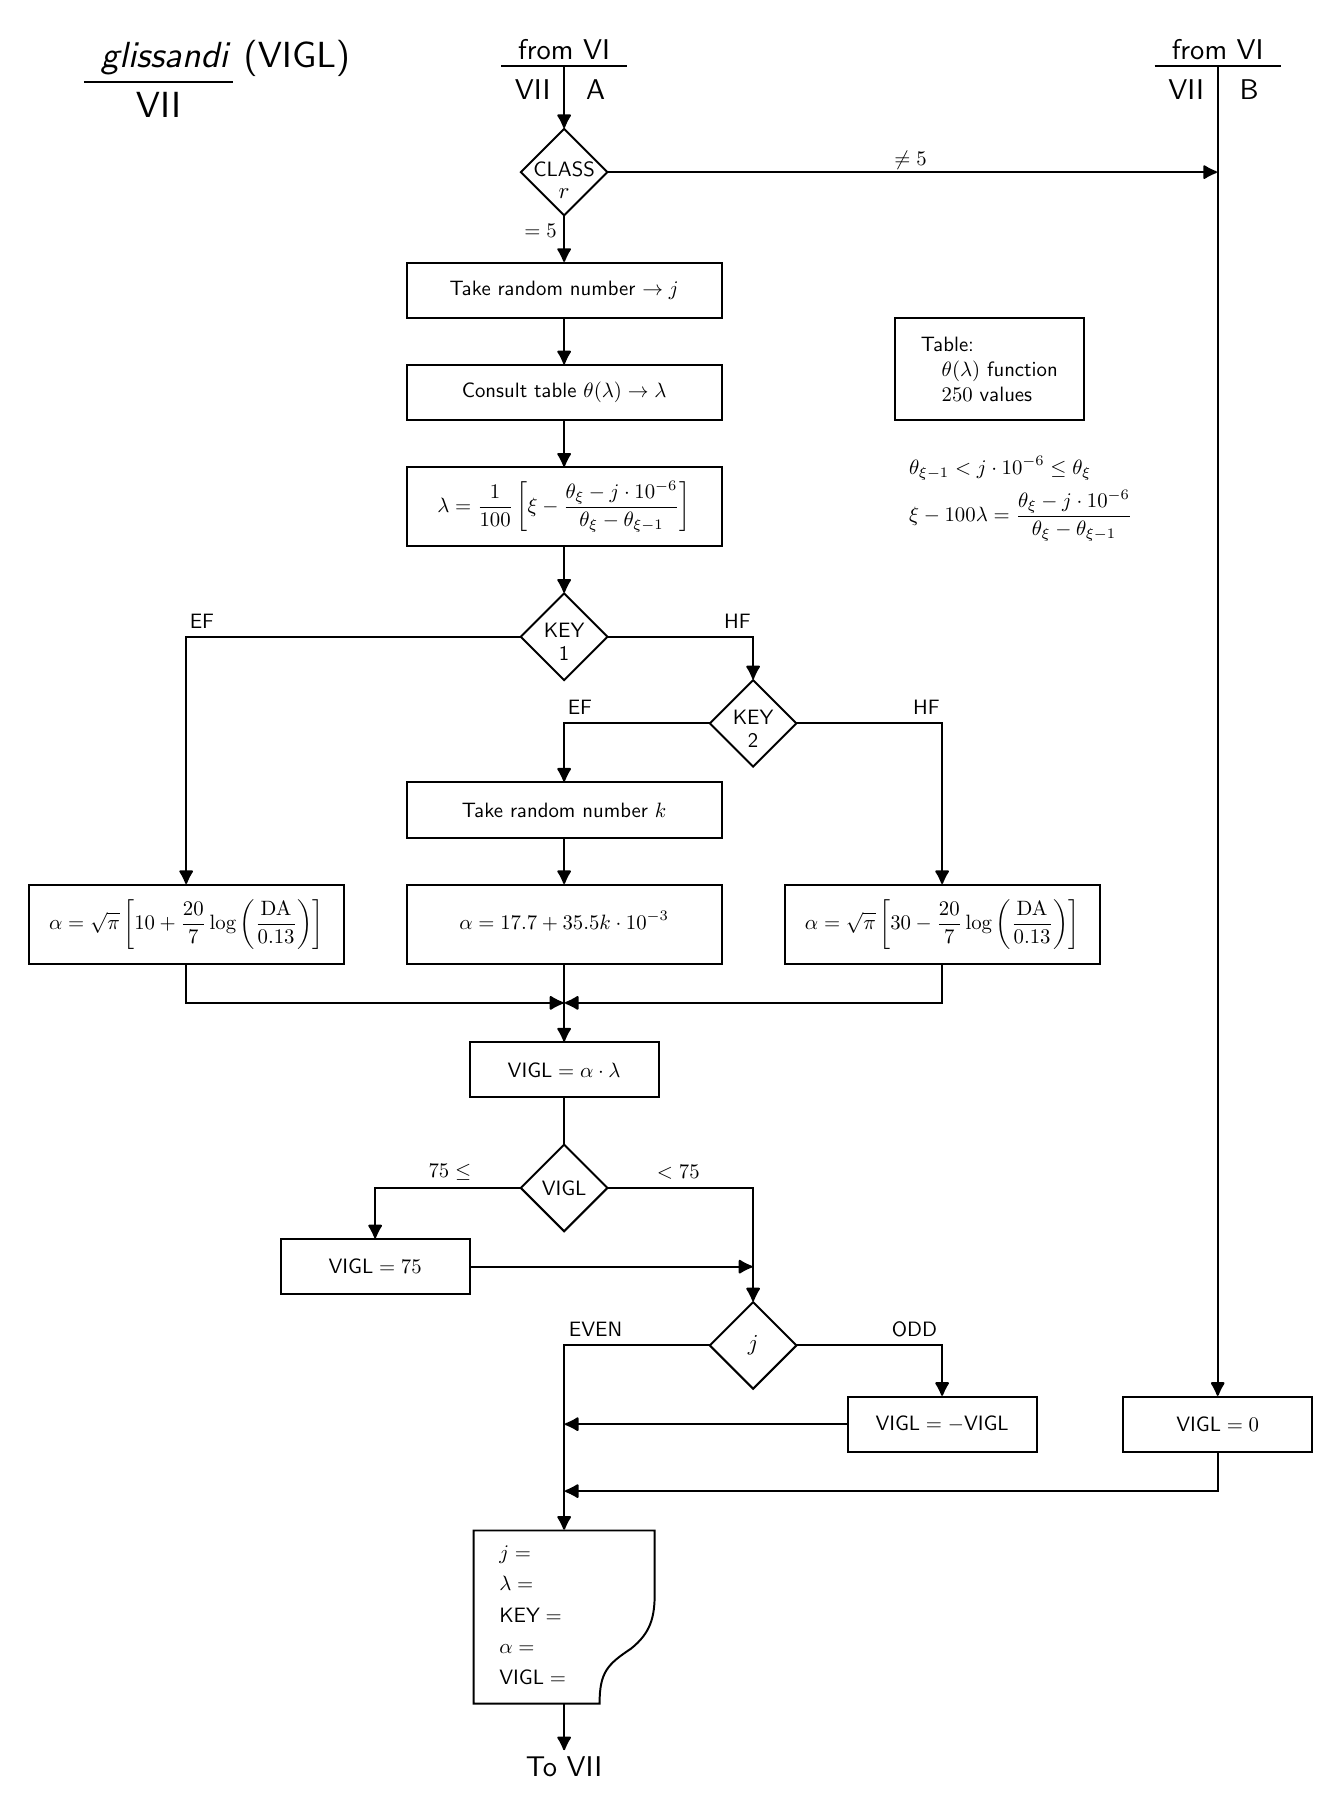
\begin{tikzpicture}[xscale=0.1,yscale=-0.1]
% yscale is set to negative due to conversion from SVG

% style
\tikzset{
    every node/.style={scale=0.75}, % assume main diagram text is 8pt
    baseLine/.style={draw, line width=0.25mm},
    arrowLine/.style={baseLine, ->, >={Latex[round, length=2mm, width=2mm]}}
}

% diamonds
\draw[baseLine] (63.5, 18.5) -- ++(5.5, -5.5) -- ++(5.5, 5.5) -- ++(-5.5, 5.5) -- cycle;
\draw[baseLine] (63.5, 77.5) -- ++(5.5, -5.5) -- ++(5.5, 5.5) -- ++(-5.5, 5.5) -- cycle;
\draw[baseLine] (87.5, 88.5) -- ++(5.5, -5.5) -- ++(5.5, 5.5) -- ++(-5.5, 5.5) -- cycle;
\draw[baseLine] (63.5,147.5) -- ++(5.5, -5.5) -- ++(5.5, 5.5) -- ++(-5.5, 5.5) -- cycle;
\draw[baseLine] (87.5,167.5) -- ++(5.5, -5.5) -- ++(5.5, 5.5) -- ++(-5.5, 5.5) -- cycle;

\node at (69, 18.2) {CLASS}; \node[scale=1.1] at (69, 21.2) {$ r $};
\node at (69, 76.7) {KEY};   \node at (69,79.7) {1};
\node at (93, 87.7) {KEY};   \node at (93,90.7) {2};
\node at (69,147.5) {VIGL};  \node[scale=1.1] at (93,167.5) {$ j $};

% rectangles
\foreach \x/\y/\w/\h in {
    49/30/40/7,
    49/43/40/7,
    111/37/24/13,
    49/56/40/10,
    49/96/40/7,
    1/109/40/10,
    49/109/40/10,
    97/109/40/10,
    57/129/24/7,
    33/154/24/7,
    105/174/24/7,
    140/174/24/7
} {
    \draw[baseLine] (\x,\y) rectangle ++(\w,\h);
}

\node at ( 69, 33.5) {Take random number $ \rightarrow j $};
\node at ( 69, 46.5) {Consult table $ \theta ( \lambda ) \rightarrow \lambda $};
\node[align=left] at (123,43.5) {Table: \\ \quad $ \theta ( \lambda ) $ function \\ \quad $ 250 $ values};
\node at ( 69, 61.0) {$ \displaystyle \lambda = \frac{1}{100} \left[ \xi - \frac{\theta_{\xi} - j \cdot 10^{-6}}{\theta_\xi - \theta_{\xi - 1}} \right] $};
\node at ( 69, 99.5) {Take random number $ k $};
\node at ( 21,114.0) {$ \displaystyle \alpha = \sqrt{\pi} \left[ 10 + \frac{20}{7} \log{\left(\frac{\mathrm{DA}}{0.13} \right)} \right] $};
\node at ( 69,113.6) {$ \displaystyle \alpha = 17.7 + 35.5k\cdot 10^{-3} $};
\node at (117,114.0) {$ \displaystyle \alpha = \sqrt{\pi} \left[ 30 - \frac{20}{7} \log{\left(\frac{\mathrm{DA}}{0.13} \right)} \right] $};
\node at ( 69,132.5) {$ \text{VIGL} = \alpha \cdot \lambda $};
\node at ( 45,157.5) {$ \text{VIGL} = 75 $};
\node at (117,177.5) {$ \text{VIGL} = -\text{VIGL} $};
\node at (152,177.5) {$ \text{VIGL} = 0 $};

% lines
\draw[baseLine] (  8,  7) -- ( 27,  7);
\draw[baseLine] ( 61,  5) -- ( 77,  5);
\draw[baseLine] (144,  5) -- (160,  5);
\draw[baseLine] ( 69,136) -- ( 69,142);

\node[scale=1.750] at ( 26,4) {\textit{glissandi} (VIGL)}; \node[scale=1.75] at (17.5,10) {VII};
\node[scale=1.375] at ( 69,3) {from VI}; \node[scale=1.375] at ( 65,8) {VII}; \node[scale=1.375] at ( 73,8) {A};
\node[scale=1.375] at (152,3) {from VI}; \node[scale=1.375] at (148,8) {VII}; \node[scale=1.375] at (156,8) {B};

% arrows
\draw[arrowLine] (69,5) -- ++(0,7.9);
\draw[arrowLine] (152,5) -- ++(0,168.9);
\draw[arrowLine] (69,24) -- ++(0,5.9);
\draw[arrowLine] (74.5,18.5) -- (151.9,18.5);
\draw[arrowLine] (69,37) -- ++(0,5.9);
\draw[arrowLine] (69,50) -- ++(0,5.9);
\draw[arrowLine] (69,66) -- ++(0,5.9);
\draw[arrowLine] (63.5,77.5) -- ++(-42.5,0) -- ++(0,31.4);
\draw[arrowLine] (74.5,77.5) -- ++(18.5,0) -- ++(0,5.4);
\draw[arrowLine] (87.5,88.5) -- ++(-18.5,0) -- ++(0,7.4);
\draw[arrowLine] (98.5,88.5) -- ++(18.5,0) -- ++(0,20.4);
\draw[arrowLine] (69,103) -- ++(0,5.9);
\draw[arrowLine] (21,119) -- ++(0,5) -- ++(47.9,0);
\draw[arrowLine] (69,119) -- ++(0,9.9);
\draw[arrowLine] (117,119) -- ++(0,5) -- ++(-47.9,0);
\draw[arrowLine] (63.5,147.5) -- ++(-18.5,0) -- ++(0,6.4);
\draw[arrowLine] (74.5,147.5) -- ++(18.5,0) -- ++(0,14.4);
\draw[arrowLine] (57,157.5) -- (92.9,157.5);
\draw[arrowLine] (87.5,167.5) -- ++(-18.5,0) -- ++(0,23.4);
\draw[arrowLine] (98.5,167.5) -- ++(18.5,0) -- ++(0,6.4);
\draw[arrowLine] (105,177.5) -- (69.1,177.5);
\draw[arrowLine] (152,181) -- ++(0,5) -- (69.1,186);
\draw[arrowLine] (69,213) -- ++(0,5.9);

\node at (66,26) {$ =5 $};
\node at (113,17) {$ \neq 5 $};
\node at (127,60) {
    $
    \begin{aligned}
        &\theta_{\xi - 1} < j \cdot 10^{-6} \leq \theta_{\xi} \\
        &\xi - 100 \lambda = \frac{\theta_{\xi} - j \cdot 10^{-6}}{\theta_\xi - \theta_{\xi - 1}}
    \end{aligned}
    $
};
\node at (23,75.5) {EF};
\node at (91,75.5) {HF};
\node at (71,86.5) {EF};
\node at (115,86.5) {HF};
\node at (54.5,145.5) {$ 75 \leq $};
\node at (83.5,145.5) {$ <75 $};
\node at (73,165.5) {EVEN};
\node at (113.5,165.5) {ODD};
\node[scale=1.375] at (69,221) {To VII};

% ending shape
\draw[baseLine]
  (57.5,191) -- ++(0,22) -- ++(16,0)
    .. controls (73.5,209) and (74.5,208) .. (77.5,206)
    .. controls (80,204)   and (80.5,202) .. (80.5,199)
    .. controls (80.5,196) and (80.5,191) .. (80.5,191)
  -- cycle;

\node at (65,202) {
    $
    \begin{aligned}
        &j = \\
        &\lambda = \\
        &\text{KEY} = \\
        &\alpha = \\
        &\text{VIGL} = \\
    \end{aligned}
    $
};

\end{tikzpicture}
}
    \caption{Excerpt from the First Flow Chart of Achorripsis}
    \label{fig:flow-chart}
\end{figure}

The statement of the thesis of \textit{Achorripsis} receives its first machine-oriented
interpretation in the following manner:

\begin{enumerate}
    \item 
        \textit{The work consists of a succession of sequences or movements each \( a_i \) seconds
        long}. Their durations are totally independent (asymmetric) but have a fixed mean duration,
        which is introduced in the form of a parameter. These durations and their stochastic
        succession are given by the formula
        \[
            P_{a_i} = c \mathrm{e}^{-ca_i} \, \mathrm{d}a_i \tag{See Appendix I.}
        \]
    \item
        \textit{Definition of the mean density of the sounds during \( a_i \)}. During a sequence
        sounds are emitted from several sonic sources. If the total number of these sounds or points
        during a sequence is \( N_{a_i} \), the mean density of this point-cluster is
        \( N_{a_i} / a_i \) sounds/sec. In general, for a given instrumental ensemble this density
        has limits that depend on the number of instrumentalists, the nature of their instruments,
        and the technical difficulties of performance. For a large orchestra the upper limit is of
        the order of \( 150 \) sounds/sec. The lower limit \( (\mathrm{V}3) \) is arbitrary and
        positive. We choose \( (\mathrm{V}3) = 0.11 \) sounds/sec. Previous experiments led us to
        adopt a logarithmic progression for the density sensation with a number between \( 2 \) and
        \( 3 \) as its base. We adopted \( \mathrm{e} = 2.71827 \). Thus the densities are included
        between \( (\mathrm{V}3)\mathrm{e}^0 \) and \( (\mathrm{V}3)\mathrm{e}^R \) sounds/sec.,
        which we can draw on a line graduated logarithmically (base
        \( \mathrm{e} \)).\footnote{\( (\mathrm{V}3)\mathrm{e}^R \) must be equal to the upper limit,
        e.g., to \(150\) sounds/sec. in the case of a large orchestra.} As our purpose is total
        independence, we attribute to each of the sequences \(a_i\) calculated in \text{1.} a
        density represented by a point drawn at random from the portion of the line mentioned above.
        However a certain concern for continuity leads us to temper the independence of the
        densities among sequences \(a_i\); to this end we introduce a certain ``memory'' from
        sequence to sequence in the following manner:

        Let \(a_{i-1}\) be a sequence of duration \(a_{i-1}\), \((\mathrm{DA})_{i-1}\) its density,
        and \(a_i\) the next sequence with duration \(a_i\) and density \((\mathrm{DA})_i\). Density
        \((\mathrm{DA})_i\) will be given by the formula:
        \[(\mathrm{DA})_i = (\mathrm{DA})_{i-1} \mathrm{e}^{\pm x}\textrm{,}\] in which \(x\) is a
        segment of line drawn at random from a line segment \(s\) of length equal to \((R - 0)\).
        The probability of \(x\) is given by
        \[P_x = \frac{2}{s} \left(1 - \frac{x}{s}\right) \, \mathrm{d}x \tag{See Appendix I.}\] and
        finally,
        \[N_{a_i} = (\mathrm{DA})_i a_i.\]
    \item 
        \textit{Composition \(Q\) of the orchestra during sequence \(a_i\)}. First the instruments
        are divided into \(r\) classes of timbres, e.g., flutes and clarinets, oboes and bassoons,
        brasses, bowed strings, pizzicati, col legno strokes, glissandi, wood, skin, and metal
        percussion instruments, etc. (See the table for \textit{Atrées}.)
        \begin{table}[htb]
            \centering
            % \caption{ \\
            % Timbre classes and instruments as on present input data}
            \caption{ Composition of the Orchestra for \textit{Atrées} (ST/10-3,060962) \\
                Timbre classes and instruments as on present input data}
            \begin{tabular}{S[table-format=2.0] ll S[table-format=2.0]}
\textit{Class} & \multicolumn{1}{c}{\textit{Timbre}} & \multicolumn{1}{c}{\textit{Instrument}}                                & \multicolumn{1}{c}{\textit{Instrument No.}} \\
\\
1              & Percussion                          & Temple-blocks                                                          & 1 {\ \textrm{--- 5}}                        \\
               &                                     & Tom-toms                                                               & 6 {\ \textrm{--- 9}}                        \\
               &                                     & Maracas                                                                & 10                                          \\
               &                                     & Susp. Cymbal                                                           & 11                                          \\
               &                                     & Gong                                                                   & 12                                          \\
2              & Horn                                & French horn                                                            & 1                                           \\
3              & Flute                               & Flute                                                                  & 1                                           \\
4              & Clarinet                            & Clarinet B                                                             & 1                                           \\
               &                                     & Bass clar. B                                                           & 2                                           \\
5              & Glissando                           & Violin                                                                 & 1                                           \\
               &                                     & Cello                                                                  & 2                                           \\
               &                                     & Trombone                                                               & 3                                           \\
6              & Tremolo                             & Flute                                                                  & 1                                           \\
               & or                                  & Clarinet Bb                                                            & 2                                           \\
               & flutter-tongue                      & Bass clar. Bb                                                          & 3                                           \\
               &                                     & French horn                                                            & 4                                           \\
               &                                     & Trumpet                                                                & 5                                           \\
               &                                     & Trombone a                                                             & 6                                           \\
               &                                     & \begin{tabular}[t]{@{}l@{}}Trombone b\\ \ \ (pedal notes)\end{tabular} & 7                                           \\
               &                                     & Violin                                                                 & 8                                           \\
               &                                     & Cello                                                                  & 9                                           \\
7              & Plucked strings                     & Violin                                                                 & 1                                           \\
               &                                     & Cello                                                                  & 2                                           \\
8              & Struck strings                      & Violin                                                                 & 1                                           \\
               &                                     & Cello                                                                  & 2                                           \\
9              & Vibraphone                          & Vibraphone                                                             & 1                                           \\
10             & Trumpet                             & Trumpet                                                                & 1                                           \\
11             & Trombone                            & Trombone a                                                             & 1                                           \\
               &                                     & \begin{tabular}[t]{@{}l@{}}Trombone b\\ \ \ (pedal notes)\end{tabular} & 2                                           \\
12             & Bowed strings                       & Violin                                                                 & 1                                           \\
               &                                     & Cello                                                                  & 2                                          
\end{tabular}
        \end{table}
        The composition of the orchestra is stochastically conceived, i.e., the distribution of the
        classes is not deterministic. Thus during a sequence of duration \(a_i\) it may happen that
        we have 80\% pizzicati, 10\% percussion, 7\% keyboard, and 3\% flute class. Under actual
        conditions the determining factor which would condition the composition of the orchestra is
        density. We therefore connect the orchestral composition with density by means of a special
        diagram. An example from \textit{ST/10-1, 080262} is shown in
        \hyperref[fig:composition]{Fig. V-2}.

        \begin{figure}[htb]
            \centering
            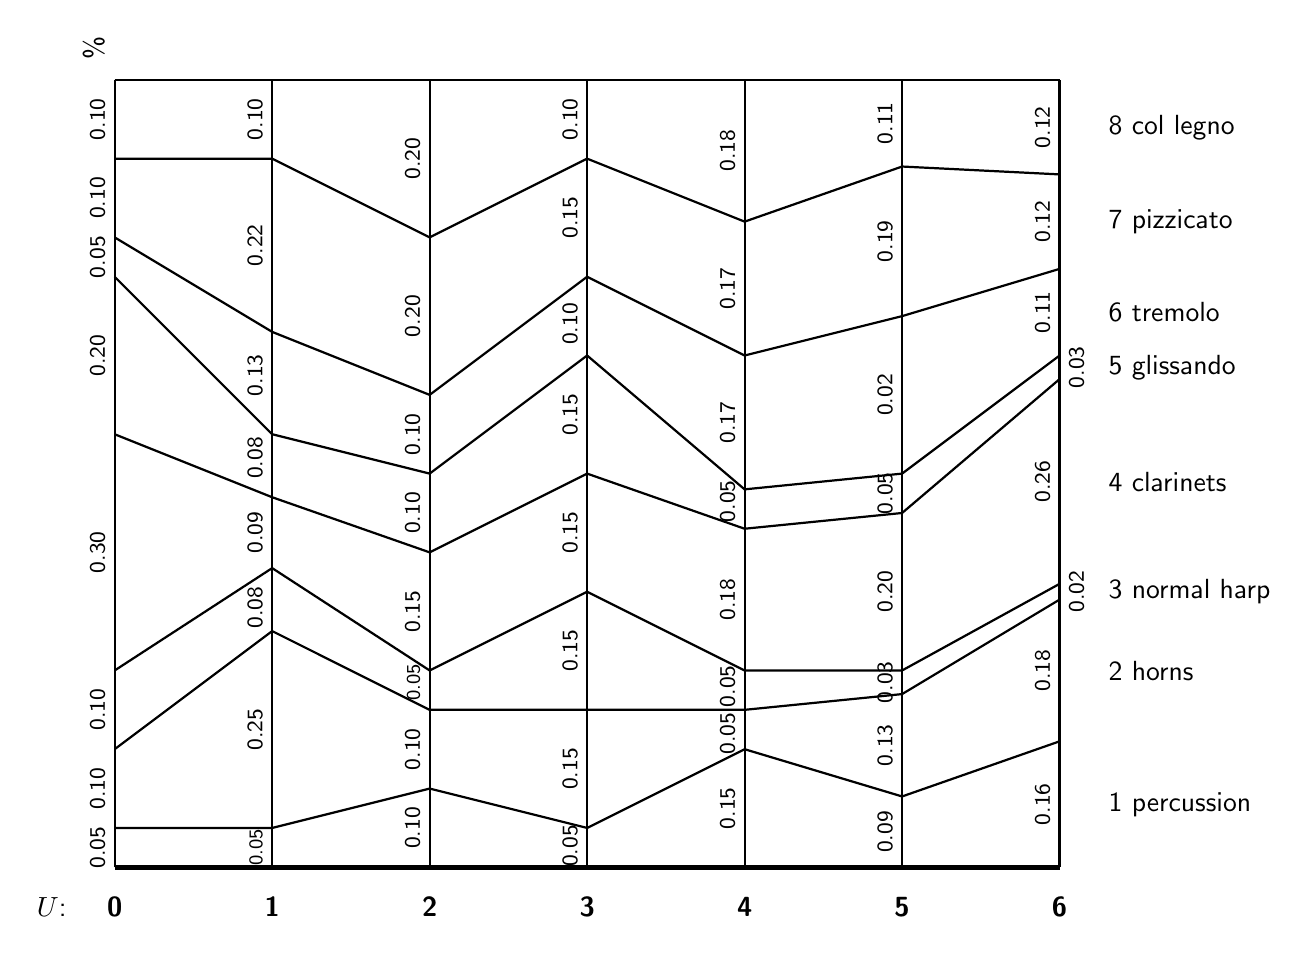
\begin{tikzpicture}[xscale=2, yscale=10]

% vertical lines
\foreach \x in {0,...,6} {
    \draw[thick] (\x, 0) -- (\x, 1);
    \node at (\x, -0.05) {\textbf{\x}};
}

% box lines
\draw[ultra thick] (0,0) -- (6,0);
\draw[thick] (0,1) -- (6,1);

% axis labels
\node at (-0.4, -0.05) {\(U\):};
\node[above, rotate=90] at (0, 1.04) {\%};

% graph lines
\draw[thick] (0,0.05) -- (1,0.05) -- (2,0.10) -- (3,0.05) -- (4,0.15) -- (5,0.09) -- (6,0.16);
\draw[thick] (0,0.15) -- (1,0.30) -- (2,0.20) -- (3,0.20) -- (4,0.20) -- (5,0.22) -- (6,0.34);
\draw[thick] (0,0.25) -- (1,0.38) -- (2,0.25) -- (3,0.35) -- (4,0.25) -- (5,0.25) -- (6,0.36);
\draw[thick] (0,0.55) -- (1,0.47) -- (2,0.40) -- (3,0.50) -- (4,0.43) -- (5,0.45) -- (6,0.62);
\draw[thick] (0,0.75) -- (1,0.55) -- (2,0.50) -- (3,0.65) -- (4,0.48) -- (5,0.50) -- (6,0.65);
\draw[thick] (0,0.80) -- (1,0.68) -- (2,0.60) -- (3,0.75) -- (4,0.65) -- (5,0.70) -- (6,0.76);
\draw[thick] (0,0.90) -- (1,0.90) -- (2,0.80) -- (3,0.90) -- (4,0.82) -- (5,0.89) -- (6,0.88);

% graph labels
\node[above, rotate=90, font=\footnotesize] at (0, 0.025) {0.05};
\node[above, rotate=90, font=\footnotesize] at (0, 0.100) {0.10};
\node[above, rotate=90, font=\footnotesize] at (0, 0.200) {0.10};
\node[above, rotate=90, font=\footnotesize] at (0, 0.400) {0.30};
\node[above, rotate=90, font=\footnotesize] at (0, 0.650) {0.20};
\node[above, rotate=90, font=\footnotesize] at (0, 0.775) {0.05};
\node[above, rotate=90, font=\footnotesize] at (0, 0.850) {0.10};
\node[above, rotate=90, font=\footnotesize] at (0, 0.950) {0.10};

\node[above, rotate=90, font=\scriptsize] at (1, 0.025) {0.05};
\node[above, rotate=90, font=\footnotesize] at (1, 0.175) {0.25};
\node[above, rotate=90, font=\footnotesize] at (1, 0.330) {0.08};
\node[above, rotate=90, font=\footnotesize] at (1, 0.425) {0.09};
\node[above, rotate=90, font=\footnotesize] at (1, 0.520) {0.08};
\node[above, rotate=90, font=\footnotesize] at (1, 0.625) {0.13};
\node[above, rotate=90, font=\footnotesize] at (1, 0.790) {0.22};
\node[above, rotate=90, font=\footnotesize] at (1, 0.950) {0.10};

\node[above, rotate=90, font=\footnotesize] at (2, 0.050) {0.10};
\node[above, rotate=90, font=\footnotesize] at (2, 0.150) {0.10};
\node[above, rotate=90, font=\scriptsize] at (2, 0.235) {0.05};
\node[above, rotate=90, font=\footnotesize] at (2, 0.325) {0.15};
\node[above, rotate=90, font=\footnotesize] at (2, 0.450) {0.10};
\node[above, rotate=90, font=\footnotesize] at (2, 0.550) {0.10};
\node[above, rotate=90, font=\footnotesize] at (2, 0.700) {0.20};
\node[above, rotate=90, font=\footnotesize] at (2, 0.900) {0.20};

\node[above, rotate=90, font=\footnotesize] at (3, 0.027) {0.05};
\node[above, rotate=90, font=\footnotesize] at (3, 0.125) {0.15};
\node[above, rotate=90, font=\footnotesize] at (3, 0.275) {0.15};
\node[above, rotate=90, font=\footnotesize] at (3, 0.425) {0.15};
\node[above, rotate=90, font=\footnotesize] at (3, 0.575) {0.15};
\node[above, rotate=90, font=\footnotesize] at (3, 0.690) {0.10};
\node[above, rotate=90, font=\footnotesize] at (3, 0.825) {0.15};
\node[above, rotate=90, font=\footnotesize] at (3, 0.950) {0.10};

\node[above, rotate=90, font=\footnotesize] at (4, 0.075) {0.15};
\node[above, rotate=90, font=\footnotesize] at (4, 0.170) {0.05};
\node[above, rotate=90, font=\footnotesize] at (4, 0.230) {0.05};
\node[above, rotate=90, font=\footnotesize] at (4, 0.340) {0.18};
\node[above, rotate=90, font=\footnotesize] at (4, 0.465) {0.05};
\node[above, rotate=90, font=\footnotesize] at (4, 0.565) {0.17};
\node[above, rotate=90, font=\footnotesize] at (4, 0.735) {0.17};
\node[above, rotate=90, font=\footnotesize] at (4, 0.910) {0.18};

\node[above, rotate=90, font=\footnotesize] at (5, 0.045) {0.09};
\node[above, rotate=90, font=\footnotesize] at (5, 0.155) {0.13};
\node[above, rotate=90, font=\footnotesize] at (5, 0.235) {0.03};
\node[above, rotate=90, font=\footnotesize] at (5, 0.350) {0.20};
\node[above, rotate=90, font=\footnotesize] at (5, 0.475) {0.05};
\node[above, rotate=90, font=\footnotesize] at (5, 0.600) {0.02};
\node[above, rotate=90, font=\footnotesize] at (5, 0.795) {0.19};
\node[above, rotate=90, font=\footnotesize] at (5, 0.945) {0.11};

\node[above, rotate=90, font=\footnotesize] at (6, 0.080) {0.16};
\node[above, rotate=90, font=\footnotesize] at (6, 0.250) {0.18};
\node[below, rotate=90, font=\footnotesize] at (6, 0.350) {0.02};
\node[above, rotate=90, font=\footnotesize] at (6, 0.490) {0.26};
\node[below, rotate=90, font=\footnotesize] at (6, 0.635) {0.03};
\node[above, rotate=90, font=\footnotesize] at (6, 0.705) {0.11};
\node[above, rotate=90, font=\footnotesize] at (6, 0.820) {0.12};
\node[above, rotate=90, font=\footnotesize] at (6, 0.940) {0.12};

% instrument labels
\node[right] at (6.25, 0.080) {1 percussion};
\node[right] at (6.25, 0.250) {2 horns};
\node[right] at (6.25, 0.350) {3 normal harp};
\node[right] at (6.25, 0.490) {4 clarinets};
\node[right] at (6.25, 0.635) {5 glissando};
\node[right] at (6.25, 0.705) {6 tremolo};
\node[right] at (6.25, 0.820) {7 pizzicato};
\node[right] at (6.25, 0.940) {8 col legno};

\end{tikzpicture}

            \caption{\textit{ST/10-1, 080262}, Composition of the Orchestra}
            % \newline \(Density = (DA)_i = 0.11 \mathrm{e}^U\), \(U = \log_e {DA/0.11}\)}
            \label{fig:composition}
        \end{figure}

        Fig. V-2 is expressed by the formula
        \[Q_r = (n-x)(e_{n,r} - e_{n+1,r}) + e_{n,r}\] in which \(r =\) the number of the class, \(x
        = \log_\mathrm{e}{\left[(\mathrm{DA})_i/(\mathrm{V}3)\right]}\), \(n = 0, 1, 2, \dots, R\),
        such that \(n \leq x \leq n + 1\), and \(e_{n,r}\) and \(e_{n+1,r}\) are the probabilities
        of class \(r\) as a function of \(n\). It goes without saying that the composition of this
        table is a precise task of great complexity and delicacy. Once these preliminaries have been
        completed, we can define, one after the other, the \(N_{a_i}\) sounds of sequence \(a_i\).
    \item
        \textit{Definition of the moment of occurrence of the sound \(N\) within the sequence
        \(a_i\)}. The mean density of the points or sounds to be distributed within \(a_i\) is \(k =
        N_{a_i} / a_i\). The formula which gives the intervals separating the sound attacks is
        \[P_t = k \mathrm{e}^{-kt} \, \mathrm{d}t. \tag{See Appendix I.}\]
    \item
        \textit{Attribution to the above sound of an instrument belonging to orchestra \(Q\), which
        has already been calculated}. First class \(r\) is drawn at random with probability \(q_r\)
        from the orchestra ensemble calculated in 3. (Consider an urn with balls of \(r\) colors in
        various proportions.) Then from within class \(r\) the number of the instrument is drawn
        according to the probability \(p_n\) given by an arbitrary table (urn with balls of \(n\)
        colors). Here also the distribution of instruments within a class is delicate and complex.
    \item
        \textit{Attribution of a pitch as a function of the instrument}. Taking as the zero point
        the lowest Bb of the piano, we establish a chromatic scale in semitones of about \(85\)
        degrees. The range \(s\) of each instrument is thus expressed by a natural number
        (distance). But the pitch \(h_u\) of a sound is expressed by a decimal number of which the
        whole number part is related to a note of the chromatic scale within the instrument's range.
        
        Just as for the density in 2., we accept a certain memory of or dependence on the preceding
        pitch played by the same instrument, so that we have
        \[h_u = h_{u-1} \pm z,\] where \(z\) is given by the probability formula
        \[P_z = \frac{2}{s} \left( 1 - \frac{z}{s} \right) \, \mathrm{d}z. \tag{See Appendix I.}\]
        \(P_z\) is the probability of the interval \(z\) taken at random from the range \(s\), and
        \(s\) is expressed as the difference between the highest and lowest pitches that can be
        played on the instrument.
    \item
        \textit{Attribution of a glissando speed if class \(r\) is characterized as a glissando}.
        The homogeneity hypotheses in Chap. I led us to the formula
        \[f(v) = \frac{2}{a \sqrt{\pi}} \mathrm{e}^{-v^2/a^2},\] and by the transformation \(v/a =
        u\) to its homologue:
        \[T(u) = \frac{2}{\sqrt{\pi}} \int_0^u \mathrm{e}^{-u^2} \, \mathrm{d}u,\] for which there
        are tables. \(f(v)\) is the probability of occurrence of the speed \(v\) (which is expressed
        in semitones/sec.); it has a parameter \(a\), which is proportional to the standard
        deviation \(s\) (\(a = s \sqrt{2}\)).

        \(a\) is defined as a function of the logarithm of the density of sequence \(a_i\) by: an
        inversely proportional function
        \[a = \sqrt{\pi} \left( 30 - \frac{20}{R} \log{[(\mathrm{DA})_i / (\mathrm{V3})]} \right),\]
        or a directly proportional function
        \[a = \sqrt{\pi} \left( 10 + \frac{20}{R} \log{[(\mathrm{DA})_i / (\mathrm{V3})]}\right),\]
        or a function independent of density
        \[a = 17.7 + 35k,\] where \(k\) is a random number between \(0\) and \(1\).

        The constants of the preceding formulae derive from the limits of the speeds that string
        glissandi may take.

        Thus for \((\mathrm{DA})_i = 145\) sounds/sec.
        \begin{align*}
            a &= 53.2 \ \text{semitones/sec.} \\
            2s &= 75 \ \text{semitones/sec.}
        \end{align*}
        and for \((\mathrm{DA})_i = 0.13\) sounds/sec.
        \begin{align*}
            a &= 17.7 \ \text{semitones/sec.} \\
            2s &= 25 \ \text{semitones/sec.}
        \end{align*}
    \item 
        \textit{Attribution of a duration \(x\) to the sounds emitted}. To simplify we establish a
        mean duration for each instrument, which is independent of tessitura and nuance.
        Consequently we reserve the right to modify it when transcribing into traditional notation.
        The following is the list of constraints that we take into account for the establishment of
        duration \(x\):
        \begin{align*}
            &G \text{, the maximum length of respiration or desired duration} \\
            &(\mathrm{DA})_i \text{, the density of the sequence} \\
            &q_r \text{, the probability of class} \ r \\
            &p_n \text{, the probability of the instrument} \ n
        \end{align*}
        Then if we define \(z\) as a parameter of a sound's duration, \(z\) could be inversely
        proportional to the probability of the occurrence of the instrument, so that
        \[z = \frac{1}{(\mathrm{DA})_i p_n q_r}.\] \(z\) will be at its maximum when
        \((\mathrm{DA})_i p_n q_r\) is at its minimum, and in this case we could choose
        \(z_{\textrm{max}} = G\).

        Instead of letting \(z_{\textrm{max}} = G\), we shall establish a logarithmic law so as to
        freeze the growth of \(z\). This law applies for any given value of \(z\).
        \[z' = G \ln{z} / \ln{z_\textrm{max}}\]

        Since we admit a total independence, the distribution of the durations \(x\) will be
        Gaussian:
        \[f(x) = \frac{1}{s \sqrt{2 \pi}} \mathrm{e}^{-(x - m)^2/(2s^2)},\]  
        where \(m\) is the arithmetic mean of the durations, \(s\) the standard deviation, and
        \begin{align*}
            m - 4.25s &= 0 \\
            m + 4.25s &= z'
        \end{align*}
        the linear system which furnishes us with the constants \(m\) and \(s\). By assuming \(u =
        (x-m)/s\sqrt{2}\) we find the function \(T(u)\), for which we consult the tables.

        Finally, the duration \(x\) of the sound will be given by the relation
        \[x = \pm us\sqrt{2} + m.\]

        We do not take into account incompatibilities between instruments, for this would needlessly
        burden the machine's program and calculation.
    \item 
        \textit{Attribution of dynamic forms to the sounds emitted}. We define four zones of mean
        intensities: *ppp*, *p*, *f*, *ff*. Taken three at a time they yield \(4^3 = 64\)
        permutations, of which \(44\) are different (an urn with 44 colors); for example, ppp<f>p.
        \begin{table}[htb]
            \centering
            \caption{Table of the 44 Intensity Forms Derived from 4 Mean Intensity Values 
            \lilyDynamics{ppp}, \lilyDynamics{p}, \lilyDynamics{f}, \lilyDynamics{ff}}
            \renewcommand{\arraystretch}{2}
\newcommand{\createDynamics}[1]{
    \lilypond[staffsize=26]{
        \new Dynamics {
            \override DynamicText.X-offset = 0
            #1
        }
        \layout {
            \context {
                \Score
                \override SpacingSpanner.spacing-increment = 6
            }
        }
    }
}

\begin{tabular}{cc}

\createDynamics{ s1\ppp\< s1\!\ppp }           & \createDynamics{ s1\f\> s1\!\p }             \\
\createDynamics{ s1\ppp\< s1\!\p }             & \createDynamics{ s1\p\< s1\!\ff }            \\
\createDynamics{ s2\ppp\< s2\!\p\> s1\!\ppp }  & \createDynamics{ s2\p\< s2\!\ff\> s1\!\p }   \\
\createDynamics{ s1\p\> s1\!\ppp }             & \createDynamics{ s1\ff\> s1\!\p }            \\
\createDynamics{ s1\ppp\< s1\!\f }             & \createDynamics{ s2\ppp\< s2\!\ff\> s1\!\f } \\
\createDynamics{ s2\ppp\< s2\!\f\> s1\!\ppp }  & \createDynamics{ s1\ppp\< s1\!\ppp }         \\
\createDynamics{ s1\f\> s1\!\ppp }             & \createDynamics{ s1\ppp\< s1\!\ppp }         \\
\createDynamics{ s1\ppp\< s1\!\ff }            & \createDynamics{ s1\ppp\< s1\!\ppp }         \\
\createDynamics{ s2\ppp\< s2\!\ff\> s1\!\ppp } & \createDynamics{ s1\ppp\< s1\!\ppp }         \\
\createDynamics{ s1\ff\> s1\!\ppp }            & \createDynamics{ s1\ppp\< s1\!\ppp }         \\
\createDynamics{ s2\ppp\< s2\!\f\> s1\!\p }    & \createDynamics{ s1\ppp\< s1\!\ppp }         \\
\createDynamics{ s2\f\> s2\!\ppp\< s1\!\p }    & \createDynamics{ s1\ppp\< s1\!\ppp }         \\
\createDynamics{ s2\p\< s2\!\f\> s1\!\ppp }    & \createDynamics{ s1\ppp\< s1\!\ppp }         \\
\createDynamics{ s2\p\> s2\!\ppp\< s1\!\f }    & \createDynamics{ s1\ppp\< s1\!\ppp }         \\
\createDynamics{ s2\ppp\< s2\!\ff\> s1\!\p }   & \createDynamics{ s1\ppp\< s1\!\ppp }         \\
\createDynamics{ s2\ff\> s2\!\ppp\< s1\!\p }   & \createDynamics{ s1\ppp\< s1\!\ppp }         \\
\createDynamics{ s2\p\> s2\!\ppp\< s1\!\ff }   & \createDynamics{ s1\ppp\< s1\!\ppp }         \\
\createDynamics{ s2\p\< s2\!\ff\> s1\!\ppp }   & \createDynamics{ s1\ppp\< s1\!\ppp }         \\
\createDynamics{ s1\p\< s1\!\p }               & \createDynamics{ s1\ppp\< s1\!\ppp }         \\
\createDynamics{ s2\p\> s2\!\ppp\< s1\!\p }    & \createDynamics{ s1\ppp\< s1\!\ppp }         \\
\createDynamics{ s1\p\< s1\!\f }               & \createDynamics{ s1\ppp\< s1\!\ppp }         \\
\createDynamics{ s2\p\< s2\!\f\> s1\!\p }      & \createDynamics{ s1\ppp\< s1\!\ppp }         \\
\end{tabular}
        \end{table}

        <!-- Table of the 44 Intensity Forms Derived from 4 Mean Intensity Values, ppp, p, f, ff -->
    \item 
        \textit{The same operations are begun again for each sound of the cluster \(N_{a_i}\)}.
    \item
        \textit{Recalculations of the same sort are made for the other sequences}.
\end{enumerate}

An extract from the sequential statement was reproduced in Fig. V-1. Now we must proceed to the
transcription into Fortran IV, a language ``understood'' by the machine (see Fig. V-3). <!-- Fig.
V-3. Stochastic Music Rewritten in Fortran IV --> <!-- Fig. V-4. Provisional Results of One Phase of
the Analysis --> <!-- Fig. V-5. Bars 1-5 of ST/10-1,080262 -->

It is not our purpose to describe the transformation of the flow chart into Fortran. However, it
would be interesting to show an example of the adaptation of a mathematical expression to machine
methods.

Let us consider the elementary law of probability (density function)
\[ f(x) \, \mathrm{d}x = c\mathrm{e}^{-cx} \, \mathrm{d}x.\] How shall we proceed in order for the
computer to give us lengths \(x\) with the probability \(f(x) \, \mathrm{d}x\)? The machine can only
draw random numbers \(y_0\) with equiprobability between \(0\) and \(1\). We shall ``modulate'' this
probability: Assume some length \(x_0\); then we have
\[\operatorname{prob}{(0 \leq x \leq x_0)} = \int_0^{x_0} f(x) \, \mathrm{d}x = 1 -
\mathrm{e}^{-cx_0} = F(x_0),\] where \(F(x_0)\) is the distribution function of \(x\). But
\[F(x_0) = \operatorname{prob}{(0 \leq y \leq y_0)} = y_0\] then
\[1 - \mathrm{e}^{-cx_0} = y_0\] and
\[x_0 = - \frac{\ln{(1 - y_0)}}{c}\] for all \(x_0 \geq 0\).

Once the program is transcribed into language that the machine's internal organization can
assimilate, a process that can take several months, we can proceed to punching the cards and setting
up certain tests. Short sections are run on the machine to detect errors of logic and orthography
and to determine the values of the entry parameters, which are introduced in the form of variables.
This is a very important phase, for it permits us to explore all parts of the program and determine
the modalities of its operation. The final phase is the decoding of the results into traditional
notation, unless an automatic transcriber is available.

\subsection*{Conclusions}

A large number of compositions of the same kind as \textit{ST/10-1, 080262} is possible for a large
number of orchestral combinations. Other works have already been written: \textit{ST/48-1, 240162},
for large orchestra, commissioned by RTF (France III); \textit{Atrées} for ten soloists; and
\textit{Morisma-Amorisima}, for four soloists.

Although this program gives a satisfactory solution to the minimal structure, it is, however,
necessary to jump to the stage of pure composition by coupling a digital-to-analogue converter to
the computer. The numerical calculations would then be changed into sound, whose internal
organization had been conceived beforehand. At this point one could bring to fruition and generalize
the concepts described in the preceding chapters.

The following are several of the advantages of using electronic computers in musical composition:

\begin{enumerate}
    \item
        The long laborious calculation made by hand is reduced to nothing. The speed of a machine
        such as the IBM-7090 is tremendous---of the order of 500,000 elementary operations/sec.
    \item
        Freed from tedious calculations the composer is able to devote himself to the general
        problems that the new musical form poses and to explore the nooks and crannies of this form
        while modifying the values of the input data. For example, he may test all instrumental
        combinations from soloists to chamber orchestras, to large orchestras. With the aid of
        electronic computers the composer becomes a sort of pilot: he presses the buttons,
        introduces coordinates, and supervises the controls of a cosmic vessel sailing in the space
        of sound, across sonic constellations and galaxies that he could formerly glimpse only as a
        distant dream. Now he can explore them at his ease, seated in an armchair.
    \item 
        The program, i.e., the list of sequential operations that constitute the new musical form,
        is an objective manifestation of this form. The program may consequently be dispatched to
        any point on the earth that possesses computers of the appropriate type, and may be
        exploited by any composer pilot.
    \item 
        Because of certain uncertainties introduced in the program, the composer-pilot can instill
        his own personality in the sonic result he obtains.
\end{enumerate}

\lstset{language=[77]Fortran, basicstyle=\ttfamily\footnotesize, keywordstyle=\color{blue}\ttfamily,
    stringstyle=\color{red}\ttfamily, commentstyle=\color{green}\ttfamily, }

\lstinputlisting{figures/fig-3-1.f}

% \begin{figure} \centering \lstinputlisting{figures/fig-3.txt} \caption{Stochastic Music Rewritten in
%     Fortran IV} \label{fig:fortran} \end{figure}

\lstinputlisting{figures/fig-4.txt}

% \begin{figure} \centering

%     \lstinputlisting{figures/fig-4.txt}
%     \caption{Provisional Results of One Phase of the Analysis}
% \end{figure}

\newpage
\lilypondfile{figures/fig-5.ly}

\newpage

\section*{Appendix I}

\begin{center}
    \Large Two Laws of Continuous Probability
\end{center}

\subsection*{First Law}

\[P_x = c \mathrm{e}^{-cx} \, \mathrm{d}x.\]

Let \(OA\) be a segment of a straight line of length \(\ell\) on which we place \(n\) points. Their
linear density is \(c = n/\ell\). Suppose that \(\ell\) and \(n\) increase indefinitely while \(c\)
remains constant. Suppose also that these points are numbered \(A_1, A_p, A_q, \dots\) and are
distributed from left to right beginning at the origin \(0\). Let
\[x_1 = A_1 A_p, \quad x_2 = A_p A_q, \quad x_3 = A_q A_r, \dots, x_i = A_s A_t.\] The probability
that the \(i\)-th segment will have a length \(x_i\) between \(x\) and \(x + dx\) is
\[P_x = c\mathrm{e}^{-cx} \, \mathrm{d}x.\]

Now the probability \(p_n\), that there will be \(n\) points on a segment \(x\) is given by the
recurrence formula
\[\frac{p_{n+1}}{p_n} = \frac{cx}{n+1} .\] Therefore \(p_1 = (cx/1)p_0\). But \(p_0 =
\mathrm{e}^{cx}\) and
\[\mathrm{e}^{-cx} = 1 - \frac{cx}{1!} + \frac{(cx)^2}{2!} - \frac{(cx)^3}{3!} + \cdots .\] If \(x\)
is very small and if we denote it by \(dx\), we have
\[p_0 = 1 - c dx + \frac{c^2 (dx)^2}{2!} - \cdots .\] Since the powers of \(dx\) are infinitely
small for high values, \(p_0 = 1 - c dx\) and \(p_1 = c dx p_0 = c dx\). Hence, the probability
\(P_x\) is composed of the probability \(p_0 = \mathrm{e}^{-cx}\), that there will be no point on
the segment \(x\), and the probability \(p_1 = c dx\), that there will be a point in \(dx\).

\subsubsection*{Approximate Calculation of the Same Probability (For Calculation by Hand)}

Let there be \( d \) points to be placed on a straight line of length \( \ell \). The linear density
is \( c = d / \ell \) points on length \( \ell \). If the lengths are expressed in units \( v \)
then \( l = av \) (\( a > 0 \)) and \( cv = d / a \) points in the unit of length \( v \).

Then \( x_i = iv \) (\( i = 0, 1, 2, 3, \dots \)), and the probability, the asymptotic limit of the
relative frequency of the segment \( x_i \), will be
\[
    \mathrm{P}_{x_i} = c \mathrm{e}^{-civ} \Delta x_i .
    \tag{1}
    \label{eq:1-1}
\]

We shall now define the quantity \( \Delta x_i \). The probability \eqref{eq:1-1} is composed of the
probability \( p_0 = \mathrm{e}^{-civ} \), that there will be no point on \( x_i \), and the
probability \( p_1 = c \Delta x_i \) that there will be a point in \( \Delta x_i \) if \( ( c \Delta
x_i )^2 \) is small enough to be ignored. Set
\[ 0 < (c \Delta x_i)^2 < w 10^{-n}, \] where \( n \) is a sufficiently large natural number; this
expression becomes
\[ 0 < \Delta x_i < c^{-1} \cdot 10^{-n/2} . \] Substitute a constant \( z \) for \( \Delta x_i \)
such that for every \( x_i \)
\[
    z \leq \Delta x_i < c^{-1} \cdot 10^{-n/2} .
    \tag{2}
    \label{eq:1-2}
\]
Then equation \eqref{eq:1-1} is written
\[
    P_{x_i} = \mathrm{e}^{-civ} \cdot cz
    \tag{3}
    \label{eq:1-3}
\]
and must satisfy the condition
\[ \sum_{i=0}^\infty cz \mathrm{e}^{-civ} = 1 ,\] or
\[ z = \frac{1}{c} \sum_{i=0}^\infty \mathrm{e}^{-civ} .\] But since \( cv > 0 \), \(
\mathrm{e}^{-cv} < 1 \), so that
\[ \sum_{i=0}^\infty \left( \mathrm{e}^{-cv} \right)^i =\frac{1}{1 = \mathrm{e}^{-cv}} \] and
finally
\[ z = \frac{1 - \mathrm{e}^{-cv}}{c} .\]

Now from \ref{eq:1-2}
\[ \frac{1 - \mathrm{e}^{-cv}}{c} < \frac{10^{-n/2}}{c} . \] Therefore
\[ 0 < \left( 1 - \mathrm{e}^{-cv} \right) < 10^{-n/2} , \] then
\[ \left( 1 - 10^{-n/2} \right) < \mathrm{e}^{-cv} < 1 \] Thus, for \( cv > 0 \) we have \(
\mathrm{e}^{-cv} < 1 \), and for \( cv < - \log{\left( 1 - 10^{-n/2} \right)} \) we have
\[ - \log{\left( 1 - 10^{-n/2} \right)} = 10^{-n/2} + \frac{10^{-(n/2)2}}{2} +
\frac{10^{-(n/2)3}}{3} +  \frac{10^{-(n/2)4}}{4} + \cdots \] and
\[ 10^{-n/2} < - \log{\left( 1 - 10^{-n/2}\right)} .\]

In order that \( \mathrm{e}^{-cv} > 1 - 10^{-n/2} \) it is therefore sufficient that
\[
    cv \leq 10^{-n/2}.
    \tag{4}
    \label{eq:1-4}
\]
Then we may take
\[
    \Delta x_i = z = \frac{1 - \mathrm{e}^{-cv}}{c}
    \tag{5}
    \label{eq:1-5}
\]
and substitute this value in formula \eqref{eq:1-1}, from which we can now set up probability
tables. Here is an example :

Let \( d = 10 \) points as mean value to be spread on a straight line segment of length \( \ell =
\qty{100}{\cm} \). We have to define \( x_i \) and \( P_{x_i} \) as a function of \( i \), given
that \( \left( c \Delta x_i \right)^2 = 10^{-4} \) is considered to be negligible.

From \eqref{eq:1-4}, \( cv = 10^{-4/2} = 0.01 \) points in \( v \). Now \( c = d / \ell = 10 / 100
points/cm \), therefore \( c = \qty{0.1}{points/\cm} \), \( v = 0.01 / 0.1 = \qty{0.1}{\cm} \), and
\( x_i = 0.1 \cdot i cm = i mm \). From \eqref{eq:1-5},
\[\Delta x_i = \frac{1 - \mathrm{e}^{-0.01}}{0.1} = (1 - 0.9905) 10 = 0.0995 = 0.1 \text{cm}. \]
From (1),
\[P_{x_i} = \mathrm{e}^{-0.01i} \cdot 0.1 \cdot 0.1 = 0.01 \cdot (0.099005)^i .\] For calculation by
machine see Chapter V.


\subsection*{Second Law}

\[ f(j) \, \mathrm{d}j = \frac{2}{a} \left( 1 - \frac{j}{a} \right) \mathrm{d}j. \]

Each variable (pitch, intensity, density, etc.) forms an interval (distance) with its predecessor.
Each interval is identified with a segment \( x \) taken on the axis of the variable. Let there be
two points \( A \) and \( B \) on this axis corresponding to the lower and upper limits of the
variable. It is then a matter of drawing at random a segment within \( AB \) whose length is
included between \( j \) and \( j + \mathrm{d} j \) for \( 0 \leq j \leq AB \). Then the probability
of this event is:
\[
    \mathrm{P}_j = f(j) \, \mathrm{d}j = \frac{2}{a} \left( 1 - \frac{j}{a} \right) \mathrm{d}j
    \tag{1}
    \label{eq:2-1}
\]
for \( a = AB \).


\subsubsection*{Approximate Definition of this Probability for Calculation by Hand}

By taking \( \mathrm{d}j \) as a constant and \( j \) as discontinuous we set \( \mathrm{d}j = c \),
\( j = iv \) with \( v = a / m \) for \( i = 0, 1, 2, 3, \dots, m \). Equation \eqref{eq:2-1}
becomes
\[
    \mathrm{P}_j = \frac{2}{a} \left( 1 - \frac{iv}{a} \right) c.
    \tag{2}
    \label{eq:2-2}
\]
But
\[
    \sum_{i=0}^{m} \mathrm{P}_j = \frac{2c}{a} (m + 1) - \frac{2cv}{a^2} \sum_{i=0}^{m} i = \frac{2c (m+1)}{a} - \frac{2cvm (m+1)}{2a^2} = 1,
\]
whence
\[ \mathrm{d}j = c = \frac{a}{m + 1} . \]

On the other hand \( \mathrm{P}_j \) must be taken as a function of the decimal approximation
required:
\[ \mathrm{P}_j = \frac{2}{m + 1} \left( 1 - \frac{i}{m} \right) \quad (n = 0, 1, 2, 3, \dots) . \]
\( P_j \) is at a maximum when \( i = 0 \), whence \( m \geq 2 \cdot 10^n - 1 \); so for \( m = 2
\cdot 10^n - 1 \) we have \( v = a / (2 \cdot 10^n - 1 ) \) and \( \mathrm{d}j = a / (2 \cdot 10^n)
\), and \eqref{eq:2-1} becomes
\[ P_j = P_i = \frac{1}{10^n} \left( 1 - \frac{i}{2 \cdot 10^n - 1} \right). \]

\subsubsection*{Definition of the Same Probability for Computer Calculation}

We know that the computer can only draw numbers \( y_0 \) at random (of equal probability) \( 0 \leq
y_0 \leq 1 \). Using the probability law of density \( P_j = f(j) \, \mathrm{d}j \), we have for
some interval \( x_0 \)
\[ \operatorname{prob.}{(0 \leq j \leq x_0)} = \int_0^{x_0} f(j) \, \mathrm{d}j = \frac{2x_0}{a} -
\frac{x_0^2}{a^2} = F(x_0), \] where \( F(x_0) \) is the distribution function of \( j \). But \(
F(x_0) = \operatorname{prob.}{(0 \leq y \leq y_0)} = y_0 \). Therefore
\[ \frac{2x_0}{a} - \frac{x_0^2}{a^2} = y_0 \quad \text{and} \quad x_0 = a \left( 1 \pm \sqrt{1 -
y_0} \right), \] and by rejecting the positive root, since \( x_0 \) must remain smaller than \( a
\), we obtain
\[ x_0 = a \left( 1 - \sqrt{1 - y_0} \right) \] for all \( 0 \leq x_0 \leq a \).

\end{document}